\documentclass[tikz,convert={outfile=\jobname.svg}]{standalone}
\usepackage{pgf} 
\usepackage{amsmath}
\usetikzlibrary{positioning}

\begin{document}
\newcommand{\drawRCC}{
  
\begin{tikzpicture}
    \fill[black] (0,0) rectangle (3, 4);
    \clip (0,0) rectangle (3, 4); 
    \fill[gray] (0, 0.2) arc[start angle=-90, end angle=90, radius=1.8] -- cycle;
    \draw[white, ultra thick] (0, 0.2) arc[start angle=-90, end angle=90, radius=1.8];
    \node[white, anchor=north east, inner sep=2, outer sep=2] at (current bounding box.north east) {RCC};
  \end{tikzpicture}
}

\newcommand{\drawMaskedRCC}[6]{
  \pgfmathsetseed{#1}
  \begin{tikzpicture}
    \fill[black] (0,0) rectangle (3, 4);
    \clip (0,0) rectangle (3, 4); 
    \fill[gray] (0, 0.2) arc[start angle=-90, end angle=90, radius=1.8] -- cycle;
    \draw[white, ultra thick] (0, 0.2) arc[start angle=-90, end angle=90, radius=1.8];
    \node[white, anchor=north east] at (3, 4) {RCC};
    \foreach \x in {0, ..., \numexpr#5-1\relax} {
      \foreach \y in {0, ..., \numexpr#6-1\relax} {
        \pgfmathsetmacro{\width}{3/#5}
        \pgfmathsetmacro{\height}{4/#6}
        \draw[white, very thin] (\x*\width, \y*\height) rectangle (\x*\width+\width, \y*\height+\height);
        \pgfmathsetmacro{\rand}{random}
        \ifdim \rand pt < \dimexpr#2 pt\relax
          \fill[#3, opacity=#4] (\x*\width, \y*\height) rectangle (\x*\width+\width, \y*\height+\height);
        \else
          \fill[black] (\x*\width, \y*\height) rectangle (\x*\width+\width, \y*\height+\height);
        \fi
      }
    }
  \end{tikzpicture}
}

\newcommand{\drawMLP}{
  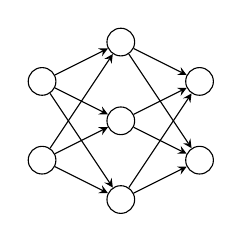
\begin{tikzpicture}
    % Input layer
    \foreach \i in {1, 2} {
      \node[circle, draw=black, fill=white, minimum size=10pt, inner sep=0pt] (input\i) at (0, -\i-0.5) {};
    }

    % Hidden layer
    \foreach \i in {1, 2, 3} {
      \node[circle, draw=black, fill=white, minimum size=10pt, inner sep=0pt] (hidden\i) at (1, -\i) {};
    }

    % Output layer
    \foreach \i in {1, 2} {
      \node[circle, draw=black, fill=white, minimum size=10pt, inner sep=0pt] (output\i) at (2, -\i-0.5) {};
    }

    % Connections from input to hidden layer
    \foreach \i in {1, 2} {
      \foreach \j in {1, 2, 3} {
        \draw[->, black, >=stealth] (input\i) -- (hidden\j);
      }
    }

    % Connections from hidden to output layer
    \foreach \i in {1, 2, 3} {
      \foreach \j in {1, 2} {
        \draw[->, black, >=stealth] (hidden\i) -- (output\j);
      }
    }
  \end{tikzpicture}
}

\newcommand{\drawFeatures}[3]{
  \begin{tikzpicture}
  \pgfmathsetseed{#1}
  \foreach \i in {0, ..., #2} {
    \node at (\i*0.8, 0) {
      $\color{#3}\scriptsize\begin{bmatrix}
        \pgfmathsetmacro{\rand}{rnd*9.9}
        \pgfmathprintnumber[fixed, precision=1]{\rand} \\
        \pgfmathsetmacro{\rand}{rnd*9.9}
        \pgfmathprintnumber[fixed, precision=1]{\rand} \\
        \vdots \\
        \pgfmathsetmacro{\rand}{rnd*9.9}
        \pgfmathprintnumber[fixed, precision=1]{\rand} \\
        \pgfmathsetmacro{\rand}{rnd*9.9}
        \pgfmathprintnumber[fixed, precision=1]{\rand}
      \end{bmatrix}$
    };
  }
  \end{tikzpicture}
}


\newcommand{\drawPosEnc}{
  \begin{tikzpicture}
  \node[circle, draw=black, minimum size=6cm, inner sep=1cm] (circle) at (0, 0) {};
  \draw[black] (-3, 0) sin (-1.5, -1) cos (0, 0) sin (1.5, 1) cos (3, 0);
  \end{tikzpicture}
}


\newcommand{\drawVector}[4]{
  % #1: number of squares
  % #2: orientation (h for horizontal, v for vertical)
  % #3: fill color
  % #4: stroke color
  \begin{tikzpicture}
    \foreach \i in {0,...,\numexpr#1-1\relax} {
      \ifthenelse{\equal{#2}{h}}{
        \fill[#3] (\i,0) rectangle (\i+1,1);
        \draw[#4] (\i,0) rectangle (\i+1,1);
      }{
        \fill[#3] (0,-\i*1) rectangle (1,-\i*1-1);
        \draw[#4] (0,-\i*1) rectangle (1,-\i*1-1);
      }
    }
  \end{tikzpicture}
}


\newcommand{\drawLayerBlock}[2]{
  % #1: Inner text
  % #2: Fill color
  \begin{tikzpicture}
    \tikzset{
        curved box/.style={
            draw,
            rounded corners=5pt,
            minimum width=1cm,
            minimum height=3cm,
            align=center,
            fill=#2
        }
    }
    \node[curved box, name=block] at (0,0) {\rotatebox{-90}{#1}};
  \end{tikzpicture}
}

\newcommand{\drawEncoderBlock}{
  \begin{tikzpicture}
    \node[name=sa] at (0, 0){\drawLayerBlock{Self Attention}{red!20}};
    \node[name=mlp] at (1.5, 0){\drawLayerBlock{MLP}{purple!20}};
    \draw[->, black, >=stealth] (sa) -- (mlp);

    \tikzset{
        curved box/.style={
            draw,
            rounded corners=5pt,
            minimum width=1cm,
            minimum height=3cm,
            align=center,
        }
    }
    \node[curved box, draw, fit=(sa) (mlp), inner sep=4pt] {};
  \end{tikzpicture}
}

\newcommand{\drawAddNode}{
  
\begin{tikzpicture}
    \node[circle, draw, minimum size=10pt] (plus) at (0,0) {$+$};
  \end{tikzpicture}
}

\newcommand{\drawDetailedEncoderBlock}{
  \begin{tikzpicture}
    \node[outer sep=1pt, inner sep=0pt] (start) {};

    % Define spacing variable
    \def\blockspacing{0.4cm}

    % Self Attention
    \node[name=norm1, right=\blockspacing of start]{\drawLayerBlock{Layer Norm}{green!20}};
    \node[name=sa, right=\blockspacing of norm1]{\drawLayerBlock{Self Attention}{red!20}};
    \node[name=scale_sa, right=\blockspacing of sa]{\drawLayerBlock{Layer Scale}{gray!20}};
    \node[name=resid1, scale=0.75, outer sep=1pt, inner sep=1pt, right=\blockspacing of scale_sa]{\drawAddNode};
    \draw[->, black, >=stealth] (start) -- (norm1);
    \draw[->, black, >=stealth] (norm1) -- (sa);
    \draw[->, black, >=stealth] (sa) -- (scale_sa);
    \draw[->, black, >=stealth] (scale_sa) -- (resid1);
    \draw[->, black, >=stealth] (start) 
        |- (norm1.north west) 
        -| (resid1.north west);

    % MLP
    \node[name=norm2, right=\blockspacing of resid1]{\drawLayerBlock{Layer Norm}{green!20}};
    \node[name=mlp, right=\blockspacing of norm2]{\drawLayerBlock{MLP}{purple!20}};
    \node[name=scale_mlp, right=\blockspacing of mlp]{\drawLayerBlock{Layer Scale}{gray!20}};
    \node[name=resid2, scale=0.75, outer sep=1pt, inner sep=1pt, right=\blockspacing of scale_mlp]{\drawAddNode};
    \draw[->, black, >=stealth] (resid1) -- (norm2);
    \draw[->, black, >=stealth] (norm2) -- (mlp);
    \draw[->, black, >=stealth] (mlp) -- (scale_mlp);
    \draw[->, black, >=stealth] (scale_mlp) -- (resid2);
    \draw[->, black, >=stealth] (resid1.north east) 
        |- (norm2.north west) 
        -| (resid2);

    % Group
    \tikzset{
        curved box/.style={
            draw,
            rounded corners=5pt,
            minimum width=1cm,
            minimum height=4cm,
            align=center,
            line width=1pt
        }
    }
    \node[curved box, draw, fit= (start) (norm1) (sa) (scale_sa) (norm2) (mlp) (scale_mlp) (resid2), inner sep=4pt] {};
  \end{tikzpicture}
}

\newcommand{\drawDecoderBlock}{
  \begin{tikzpicture}
    \node[name=sa] at (0, 0){\drawLayerBlock{Self Attention}{red!20}};
    \node[name=ca] at (1.5, 0){\drawLayerBlock{Cross Attention}{green!20}};
    \node[name=mlp] at (3, 0){\drawLayerBlock{MLP}{purple!20}};
    \draw[->, black, >=stealth] (sa) -- (ca);
    \draw[->, black, >=stealth] (ca) -- (mlp);

    \tikzset{
        curved box/.style={
            draw,
            rounded corners=5pt,
            minimum width=1cm,
            minimum height=3cm,
            align=center,
        }
    }
    \node[curved box, draw, fit=(sa) (ca) (mlp), inner sep=4pt] {};
  \end{tikzpicture}
}

\newcommand{\drawConv}[3]{
  % #1: kernel size
  % #2: color
  % #3: filter count
  \begin{tikzpicture}
    % Draw the stacked filters with perspective
    \foreach \i in {0,...,#3} {
      \begin{scope}[yshift=\i*5pt]
        \foreach \x in {0,...,\numexpr#1-1\relax} {
          \foreach \y in {0,...,\numexpr#1-1\relax} {
            \draw[fill=#2] (\x*0.2,\y*0.2) rectangle ++(0.2,0.2);
          }
        }
      \end{scope}
    }
  \end{tikzpicture}
}


\newcommand{\drawDetailedDecoderBlock}[1]{
  % #1: t to use self attn, f to not use self attn
  \begin{tikzpicture}
    \node[outer sep=1pt, inner sep=0pt] (start) {};

    % Define spacing variable
    \def\blockspacing{0.4cm}

    % Self Attention (only if #1 is t)
    \ifthenelse{\equal{#1}{t}}{
      \node[name=norm1, right=\blockspacing of start]{\drawLayerBlock{Layer Norm}{green!20}};
      \node[name=sa, right=\blockspacing of norm1]{\drawLayerBlock{Self Attention}{red!20}};
      \node[name=scale_sa, right=\blockspacing of sa]{\drawLayerBlock{Layer Scale}{gray!20}};
      \node[name=resid1, scale=0.75, outer sep=1pt, inner sep=1pt, right=\blockspacing of scale_sa]{\drawAddNode};
      \draw[->, black, >=stealth] (start) -- (norm1);
      \draw[->, black, >=stealth] (norm1) -- (sa);
      \draw[->, black, >=stealth] (sa) -- (scale_sa);
      \draw[->, black, >=stealth] (scale_sa) -- (resid1);
      \draw[->, black, >=stealth] (start) 
          |- (norm1.north west) 
          -| (resid1.north west);
    }{
      \node[name=resid1] at (start) {};
    }

    % Cross Attention
    \node[name=norm2, right=\blockspacing of resid1]{\drawLayerBlock{Layer Norm}{green!20}};
    \node[name=ca, right=\blockspacing of norm2]{\drawLayerBlock{Cross Attention}{blue!20}};
    \node[name=scale_ca, right=\blockspacing of ca]{\drawLayerBlock{Layer Scale}{gray!20}};
    \node[name=resid2, scale=0.75, outer sep=1pt, inner sep=1pt, right=\blockspacing of scale_ca]{\drawAddNode};
    \draw[->, black, >=stealth] (resid1) -- (norm2);
    \draw[->, black, >=stealth] (norm2) -- (ca);
    \draw[->, black, >=stealth] (ca) -- (scale_ca);
    \draw[->, black, >=stealth] (scale_ca) -- (resid2);
    \ifthenelse{\equal{#1}{t}}{
      \draw[->, black, >=stealth] (resid1.north east) 
          |- (norm2.north west) 
          -| (resid2);
    }{
      \draw[->, black, >=stealth] (start.north east)
          |- (norm2.north west)
          -| (resid2);
    }

    % MLP
    \node[name=norm3, right=\blockspacing of resid2]{\drawLayerBlock{Layer Norm}{green!20}};
    \node[name=mlp, right=\blockspacing of norm3]{\drawLayerBlock{MLP}{purple!20}};
    \node[name=scale_mlp, right=\blockspacing of mlp]{\drawLayerBlock{Layer Scale}{gray!20}};
    \node[name=resid3, scale=0.75, outer sep=1pt, inner sep=1pt, right=\blockspacing of scale_mlp]{\drawAddNode};
    \draw[->, black, >=stealth] (resid2) -- (norm3);
    \draw[->, black, >=stealth] (norm3) -- (mlp);
    \draw[->, black, >=stealth] (mlp) -- (scale_mlp);
    \draw[->, black, >=stealth] (scale_mlp) -- (resid3);
    \draw[->, black, >=stealth] (resid2.north east) 
        |- (norm3.north west) 
        -| (resid3);

    % Group
    \tikzset{
        curved box/.style={
            draw,
            rounded corners=5pt,
            minimum width=1cm,
            minimum height=4cm,
            align=center,
            line width=1pt
        }
    }
    \node[curved box, draw, fit= (start) (norm2) (ca) (scale_ca) (norm3) (mlp) (scale_mlp) (resid3), inner sep=4pt] {};

    % Anchors
    \coordinate (ca_north) at (ca.north);
    \coordinate (ca_south) at (ca.south);
    \coordinate (ca_east) at (ca.east); 
    \coordinate (ca_west) at (ca.west);
  \end{tikzpicture}
}
\tikzset{every picture/.style={/utils/exec={\sffamily}}}

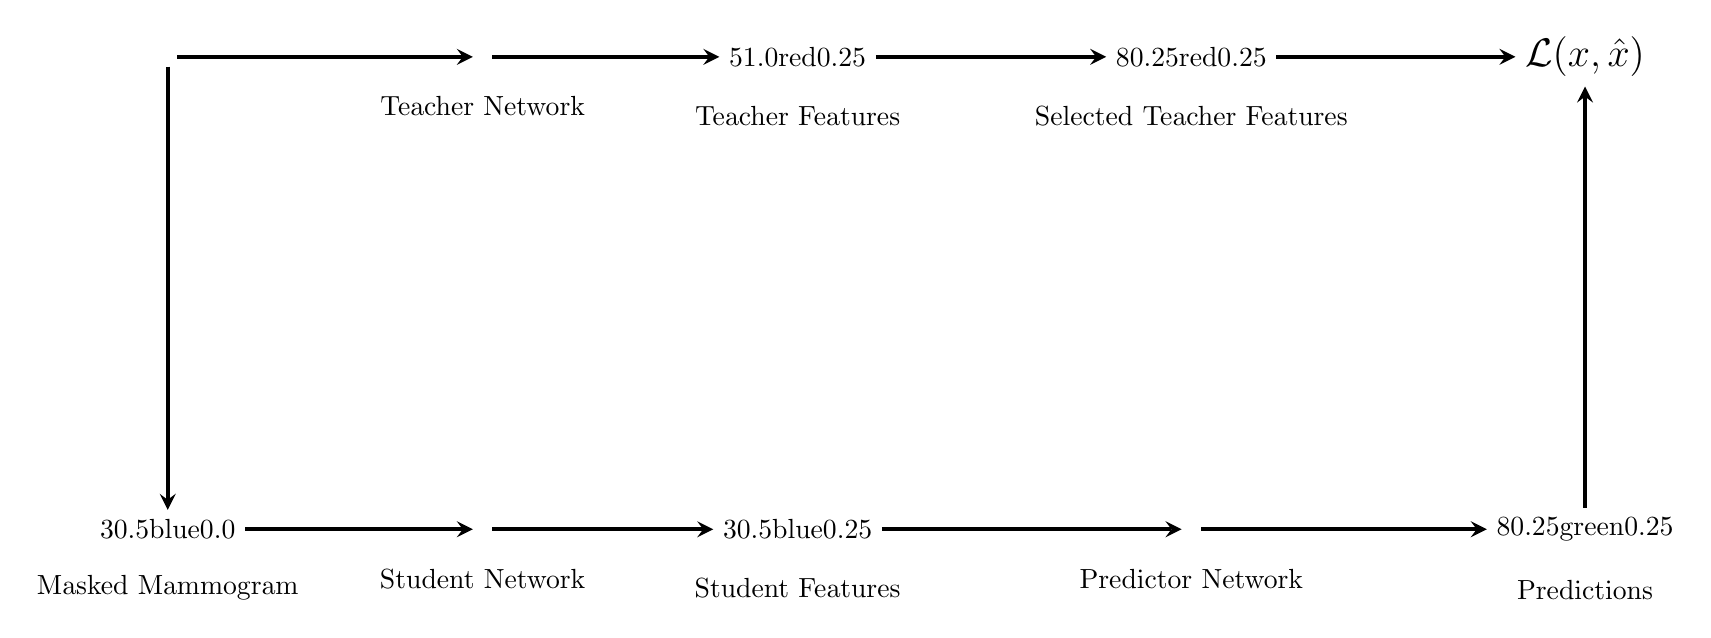
\begin{tikzpicture}

  % Innput mammogram
  \node[name=rcc] at (0, 0){\drawRCC};

  % Teacher network 
  \node[name=teacher] at (4, 0){\drawMLP};
  \node[below=0.5cm of teacher.south, anchor=center] {Teacher Network};
  \draw[->, thick, black, >=stealth, line width=1.5pt] (rcc) -- (teacher);

  % Masked mammogram
  \node[name=masked_rcc] at (0, -6){\drawMaskedRCC{3}{0.5}{blue}{0.0}};
  \node[below=0.5cm of masked_rcc.south, anchor=center] {Masked Mammogram};
  \draw[->, thick, black, >=stealth, line width=1.5pt] (rcc) -- (masked_rcc);

  % Student network
  \node[name=student] at (4, -6){\drawMLP};
  \node[below=0.5cm of student.south, anchor=center] {Student Network};
  \draw[->, thick, black, >=stealth, line width=1.5pt] (masked_rcc) -- (student);

  % Student features
  \node[name=student_features] at (8, -6){\drawMaskedRCC{3}{0.5}{blue}{0.25}};
  \node[below=0.5cm of student_features.south, anchor=center] {Student Features};
  \draw[->, thick, black, >=stealth, line width=1.5pt] (student) -- (student_features);

  % Teacher features
  \node[name=teacher_features] at (8, 0){\drawMaskedRCC{5}{1.0}{red}{0.25}};
  \node[below=0.5cm of teacher_features.south, anchor=center] {Teacher Features};
  \draw[->, thick, black, >=stealth, line width=1.5pt] (teacher) -- (teacher_features);

  % Masked teacher features
  \node[name=masked_teacher_features] at (13, 0){\drawMaskedRCC{8}{0.25}{red}{0.25}};
  \node[below=0.5cm of masked_teacher_features.south, anchor=center] {Selected Teacher Features};
  \draw[->, thick, black, >=stealth, line width=1.5pt] (teacher_features) -- (masked_teacher_features);

  % Predictor
  \node[name=predictor] at (13, -6){\drawMLP};
  \node[below=0.5cm of predictor.south, anchor=center] {Predictor Network};
  \draw[->, thick, black, >=stealth, line width=1.5pt] (student_features) -- (predictor);

  % Positions
  %\draw[->, thick, black, >=stealth, line width=1.5pt] (teacher_features.east) to[out=0, in=180] node[midway, right] {Selected Positions} (predictor.west);

  % Predictions
  \node[name=predictions] at (18, -6){\drawMaskedRCC{8}{0.25}{green}{0.25}};
  \node[below=0.5cm of predictions.south, anchor=center] {Predictions};
  \draw[->, thick, black, >=stealth, line width=1.5pt] (predictor) -- (predictions);

  % Loss
  \node[name=loss] at (18, 0){\Large $\mathcal{L}(x, \hat{x})$};

  % Arrows to loss
  \draw[->, thick, black, >=stealth, line width=1.5pt] (masked_teacher_features) to[out=0, in=180] (loss);
  \draw[->, thick, black, >=stealth, line width=1.5pt] (predictions.north) to[out=90, in=270] (loss);


\end{tikzpicture}
\end{document}